\documentclass[citecolor=blue,10pt]{beamer}
\usepackage{graphicx, color, booktabs}
\usepackage{lmodern}
\usepackage{natbib}
\usepackage{fancybox}
\usepackage{marvosym}
\usepackage{algorithm}
\usepackage{algorithmic}
%\usepackage{bbding}
%\usepackage[citecolor=blue]{hyperref}
\usepackage{textpos}
\hypersetup{
  colorlinks,
  citecolor=blue,
  linkcolor=black
}



%% maxwidth is the original width if it is less than linewidth
%% otherwise use linewidth (to make sure the graphics do not exceed the margin)

%\addtobeamertemplate{frametitle}{}{%
%\begin{textblock*}{200mm}(.8\textwidth,-0.5cm)
%\includegraphics[height=1cm,width=3cm]{ksu}
%\end{textblock*}}


\def\I{\mathbb{I}}

\def\bg{{\boldsymbol \gamma}}
\definecolor{fgcolor}{rgb}{0.2, 0.2, 0.2}
\def\R{\mathbb{R}}
\def\T{{ \mathrm{\scriptscriptstyle T} }}
\def\v{{\varepsilon}}
\def\uSigma{{\boldsymbol \Sigma}}
\newcommand{\uone} {\mbox{\boldmath$1$}}
\newcommand{\0} {\mbox{\boldmath$0$}}
\newcommand{\uV} {{\boldsymbol V}}
\newcommand{\uv} {\mbox{\boldmath$v$}}
\newcommand{\uu} {\mbox{\boldmath$u$}}
\newcommand{\uH} {{\boldsymbol H}}
\newcommand{\uB} {{\boldsymbol B}}
\newcommand{\uD} {{\boldsymbol D}}
\newcommand{\uU} {{\boldsymbol U}}
\newcommand{\uC} {\mbox{\boldmath$C$}}
\newcommand{\uE} {\mbox{\boldmath$E$}}
\newcommand{\pkg}[1]{{\fontseries{b}\selectfont #1}} 
\newcommand{\uA}{{\boldsymbol A}}
\newcommand{\ua}{{\boldsymbol a}}
\newcommand{\uz}{{\boldsymbol z}}
\newcommand{\ub}{{\boldsymbol b}}
\newcommand{\uy}{{\boldsymbol y}}
\newcommand{\uo}{{\boldsymbol o}}
\newcommand{\uc}{{\boldsymbol c}}
\newcommand{\uY}{{\boldsymbol Y}}
\newcommand{\ux}{{\boldsymbol x}}
\newcommand{\uh}{{\boldsymbol h}}

\newcommand{\uX}{{\boldsymbol X}}
\newcommand{\uw} {\mbox{\boldmath$w$}}

\newcommand{\ug} {\mbox{\boldmath$g$}}
\newcommand{\uW} {\mbox{\boldmath$W$}}
\newcommand{\us} {\mbox{\boldmath$s$}}
\newcommand{\um} {\mbox{\boldmath$m$}}
\newcommand{\uF} {\mbox{\boldmath$F$}}
\newcommand{\uf} {\mbox{\boldmath$f$}}
\newcommand{\udelta} {\mbox{\boldmath$\delta$}}
\newcommand{\uDelta} {\mbox{\boldmath$\Delta$}}
\newcommand{\up} {{\boldsymbol p}}
\newcommand{\uP} {\mbox{\boldmath$P$}}
\newcommand{\uQ} {\mbox{\boldmath$Q$}}

\newcommand{\uK} {\mbox{\boldmath$K$}}
\newcommand{\uZ} {\mbox{\boldmath$Z$}}
\newcommand{\uI} {\mbox{\boldmath$I$}}
\newcommand{\utheta}{{\boldsymbol \theta}}

\newcommand{\uTheta} {\mbox{\boldmath $\Theta$}}
\newcommand{\umu} {{\boldsymbol \mu}}
\newcommand{\usig} {\mbox{\boldmath $\Sigma$}}
\newcommand{\ualpha} {\mbox{\boldmath $\alpha$}}
\newcommand{\ulambda}{{\boldsymbol \lambda}}
\newcommand{\ubeta}{{\boldsymbol \beta}}
\newcommand{\ueta} {\mbox{\boldmath $\eta$}}
\newcommand{\utau} {\mbox{\boldmath $\tau$}}
\newcommand{\ukappa} {\mbox{\boldmath $\kappa$}}
\newcommand{\uepsilon} {\mbox{\boldmath $\epsilon$}}
\newcommand{\uOmega} {\mbox{\boldmath $\Omega$}}
\renewcommand{\bibsection}{\vskip 5mm\centering{REFERENCES}}
\newcommand{\red}{\textcolor{red}}
\newcommand{\card}{{\rm card}}
\newcommand{\rank}{{\rm rank}}
\def\Sup{\operatornamewithlimits{sup\vphantom{p}}}
\def\mis{{\rm mis}}
\def\obs{{\rm obs}}
\def\full{{\rm full}}
\newcommand{\Nor}{\mathcal{N}}
\newcommand{\To}{\rightarrow}
\newcommand{\Car}{\mathds{1}}
\newcommand{\Inte}{\mathds{N}}
\newcommand{\LL}{\mathds{L}}
\newcommand{\Real}{\mathds{R}}
\newcommand{\Inter}{\mathds{Z}}
\newcommand{\Esp}{\mathds{E}}
\newcommand{\Var}{\mbox{Var}}
\newcommand{\Cov}{\mbox{Cov}}
\newcommand{\Probability}{\mathbb{P}}
\newcommand{\Loi}{\mathcal{L}}
\newcommand{\Dist}{\mathcal{D}}
%\newcommand{\bfS}{\mathbf{S}}
\newcommand{\bgamma}{\mbox{\boldmath $\gamma$}}
\newcommand{\bGamma}{\mbox{\boldmath $\Gamma$}}
\newcommand{\dint}{\displaystyle\int}
%\renewcommand{\thesection}{\arabic{section}}
%\renewcommand{\theequation}{\arabic{section}.\arabic{equation}}
%\renewcommand{\thetheorem}{\arabic{section}.\arabic{theorem}}
%\renewcommand{\theassumption}{\arabic{section}.\arabic{assumption}}
%\renewcommand{\theproposition}{\arabic{section}.\arabic{proposition}}
%\renewcommand{\thecorollary}{\arabic{section}.\arabic{corollary}}
%\renewcommand{\thelemma}{\arabic{section}.\arabic{lemma}}
%\renewcommand{\theexample}{\arabic{section}.\arabic{example}}
%\renewcommand{\theremark}{\arabic{section}.\arabic{remark}}
%\renewcommand{\thealgorithm}{\arabic{section}.\arabic{algorithm}}


\usepackage{framed}
\newtheorem{proposition}{Proposition}
\newtheorem{remark}{Remark}
\newtheorem{definition1}{What is BIG DATA?}
\newtheorem{remark1}{Big Data Challenge I}
\newtheorem{remark7}{Big Data Challenge II}
\newtheorem{remark2}{Bayesian perspective}
\newtheorem{remark3}{Data}
\newtheorem{remark4}{\textcolor{red}{Generalized} Bregman divergence clustering}
\newtheorem{remark5}{Bayesian clustering with high-dimensional covariates}
\newtheorem{remark6}{Bayesian functional clustering with high-dimensional covariates}
\definecolor{shadecolor}{rgb}{.97, .97, .97}
\definecolor{messagecolor}{rgb}{0, 0, 0}
\definecolor{warningcolor}{rgb}{1, 0, 1}
\definecolor{errorcolor}{rgb}{1, 0, 0}

\usepackage{alltt}
\mode<presentation>
\setbeamercovered{dynamic}
\usetheme{Boadilla}

\begin{document}
\title{Bayesian Approaches for High-Dimensional
Data Analysis}
\author{\bf Gyuhyeong Goh}

\institute{Department of Statistics\\
Kansas State University, Manhattan, KS\\
\quad\\
\quad\\
{\color{blue} Joint work with} \\
\quad\\
{ Shiqiang Jin}\\ \quad\\ Kansas State University, Manhattan, KS
}

\date{}

\begin{frame}
\titlepage
\end{frame}

%\begin{frame}<beamer>
%\frametitle{Outline}
%\tableofcontents
%\end{frame}

\section{Introduction}

\begin{frame}{Introduction}{Data structure}
\begin{itemize}
\item In practice, we frequently observe the following data structure: 
\end{itemize}

\begin{eqnarray*}
\begin{array}{c|c|c|c|c}
Y&X_1&X_2&\cdots &X_p\\
\hline
y_1& x_{11} & x_{12}&\cdots & x_{1p}  \\
y_2& x_{21} & x_{22}&\cdots & x_{2p} \\
\vdots& \vdots & \vdots&\ddots & \vdots \\
y_n& x_{n1} & x_{n2}&\cdots & x_{np} \\
\end{array}
\end{eqnarray*}
\begin{itemize}
\item[]\quad where $Y$ is the response and $X_1,X_2,\ldots, X_p$ are the predictors.
\item We are interested in modeling the relationship between $X_1,\ldots, X_p$ and $Y$.  
\end{itemize}
\end{frame}

\begin{frame}{Introduction}{Statistical models}
\begin{itemize}
\item Regression models play an important role in many application domains for analyzing or predicting a response based on multiple predictors.
\vspace{5mm}

\begin{itemize}
\item Linear regression:
$$Y=\beta_0+\beta_1 X_1+\beta_2 X_2+\cdots +\beta_p X_p +\epsilon$$
\item Logistic regression:
$$P(Y=1)=\frac{\exp(\beta_0+\beta_1 X_1+\beta_2 X_2+\cdots +\beta_p X_p)}{1+\exp(\beta_0+\beta_1 X_1+\beta_2 X_2+\cdots +\beta_p X_p)} $$
\item Cox regression:
$$h(Y)= h_0(Y)\exp(\beta_0+\beta_1 X_1+\beta_2 X_2+\cdots +\beta_p X_p)$$
\end{itemize}
\end{itemize}

\end{frame}


\begin{frame}{Introduction}{Variable selection}
\begin{itemize}
\item \emph{Variable selection} is the process of selecting a subset of relevant predictors in regression analysis. (e.g., BIC, AIC, CV, $R^2_a$, $C_p$, ...)
\end{itemize}
\begin{figure}
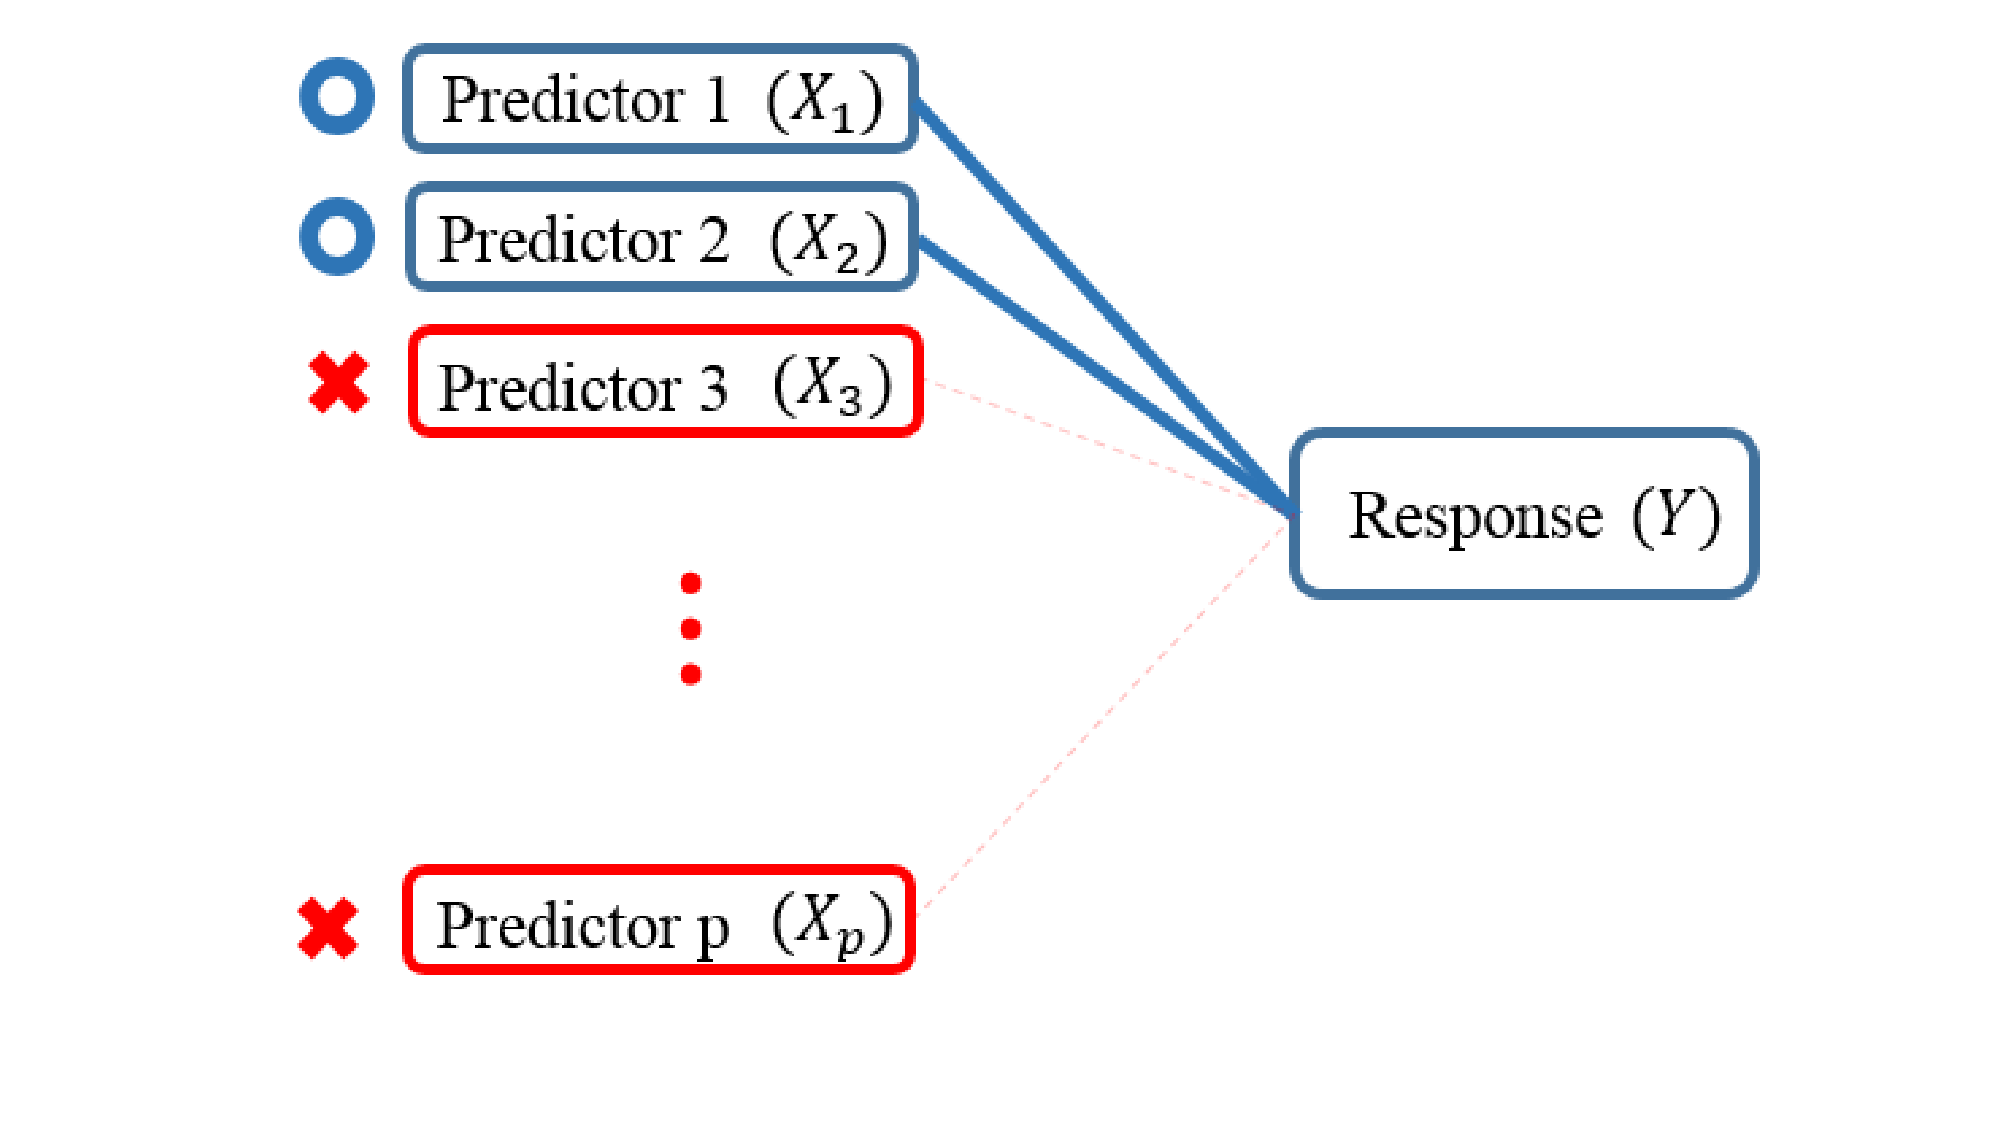
\includegraphics[width=0.8\textwidth]{Figure1.pdf}
\end{figure}
\end{frame}

\begin{frame}{Introduction}{Challenges of high-dimensional variable selection}
\begin{itemize}\itemsep=3mm
\item There are $2^p$ candidate models\\
\item[] e.g., for $p=3$
{\footnotesize
\begin{eqnarray*}
\texttt{Model 1}:\quad Y&=&\beta_0+\epsilon\\
\texttt{Model 2}:\quad Y&=&\beta_0+\beta_1X_1+\epsilon\\
\texttt{Model 3}:\quad Y&=&\beta_0+\beta_2X_2+\epsilon\\
\texttt{Model 4}:\quad Y&=&\beta_0+\beta_3X_3+\epsilon\\
\texttt{Model 5}:\quad Y&=&\beta_0+\beta_1X_1+\beta_2X_2+\epsilon\\
\texttt{Model 6}:\quad Y&=&\beta_0+\beta_1X_1+\beta_3X_3+\epsilon\\
\texttt{Model 7}:\quad Y&=&\beta_0+\beta_2X_2+\beta_3X_3+\epsilon\\
\texttt{Model 8}:\quad Y&=&\beta_0+\beta_1X_1+\beta_2X_2+\beta_3X_3+\epsilon
\end{eqnarray*}}\pause
\item When \textcolor{red}{$p$ is large}, it is \textcolor{red}{challenging to find the best subset}.
\item[]  e.g., $2^{40}\approx 1,000,000,000,000$.
\end{itemize}
\end{frame}

\begin{frame}{Introduction}{Connection between sparse estimation and variable selection}
\begin{itemize}
\item Variable selection is equivalent to estimating sparse coefficients.
\begin{itemize}
\item Linear regression:
{\footnotesize
\begin{eqnarray*}
Y&=&\beta_0+\beta_1 X_1+\beta_2 X_2 +\epsilon\\
&\Updownarrow&\\
 Y&=&\beta_0+\beta_1 X_1+\beta_2 X_2+\textcolor{red}{0} X_3+\cdots + \textcolor{red}{0} X_p +\epsilon
\end{eqnarray*}}
\item Logistic regression:
{\footnotesize
\begin{eqnarray*}
P(Y=1)&=&\frac{\exp(\beta_0+\beta_1 X_1+\beta_2 X_2)}{1+\exp(\beta_0+\beta_1 X_1+\beta_2 X_2)} \\
&\Updownarrow&\\
P(Y=1)&=&\frac{\exp(\beta_0+\beta_1 X_1+\beta_2 X_2+\textcolor{red}{0} X_3+\cdots + \textcolor{red}{0} X_p)}{1+\exp(\beta_0+\beta_1 X_1+\beta_2 X_2+\textcolor{red}{0} X_3+\cdots + \textcolor{red}{0} X_p)} 
\end{eqnarray*}}

\end{itemize}
\item Hence, variable selection can be done by producing \textcolor{red}{sparse} estimator of coefficients.
\end{itemize}

\end{frame}
\begin{frame}{High-dimensional linear regression models}
\begin{itemize}\itemsep=5mm
\item Define
\begin{eqnarray*}
\left[\begin{array}{c|cccc}
y_1& x_{11} & x_{12}&\cdots & x_{1p}  \\
y_2& x_{21} & x_{22}&\cdots & x_{2p} \\
\vdots& \vdots & \vdots&\ddots & \vdots \\
y_n& x_{n1} & x_{n2}&\cdots & x_{np} \\
\end{array}\right]=\left[\begin{array}{c|cccc}
\uy& \ux_{1} & \ux_{2}&\cdots & \ux_{p}  \\
\end{array}\right]
\end{eqnarray*}
\item Consider 
$$ \uy=\uX\ubeta +\uepsilon,$$
where $\uX=(\ux_1,\ldots,\ux_p)$, $\ubeta=(\beta_1,\ldots, \beta_p)^\T$, and $\uepsilon \sim N(0,\sigma^2 I_n)$.
 \item Assume that $p>n$.
 \item Our aim is to obtain a sparse estimator for $\ubeta$.
\end{itemize}
\end{frame}



\begin{frame}{Sparse estimation with $L_0$-penalty}
\begin{itemize}\itemsep=6mm

 \item The sparse  estimator can be obtained by minimizing 
 $$ \|\uy-\uX\ubeta\|^2 +\lambda \|\ubeta\|_0,$$
 where $\|\ubeta\|_0=\sum_{j=1}^p \mathbb{I}(\beta_j\neq 0)$ and $\lambda \geq 0$ controls degrees of sparsity.
 \item e.g., $\lambda=2$ (AIC), $\lambda=\log n$ (BIC), $\lambda =\log p $ (RIC), \ldots
 \pause \item However, the use of $L_0$-penalty leads to a \textcolor{red}{non-convex optimization} problem, which is computationally intractable in high-dimensional settings.
\end{itemize}
\end{frame}

\begin{frame}{Sparse estimation with convex penalties}
\begin{itemize}\itemsep=5mm
\item Many convex penalty functions have been proposed. 
\\e.g., lasso, adaptive lasso, elastic net, MCP, ... 
\item The lasso estimator \citep{tibshirani1996regression} can be obtained by minimizing 
 $$ \|\uy-\uX\ubeta\|^2 +\lambda \|\ubeta\|_1,$$
 where $\|\ubeta\|_1=\sum_{j=1}^p |\beta_j|$.
\pause \item However, optimal $\lambda$ selection is required. (CV, GCV, BIC, ...)
 
 \item In addition, convex penalties generate the shrinkage bias on the resulting estimator of $\ubeta$. 
\end{itemize}
\end{frame}
\begin{frame}{$L_0$-penalty vs Convex penalties} 
\begin{table}[ht]
\centering
\begin{tabular}{rrr}
  \hline
 &$L_0$-penalty & Convex penalties \\ 
  \hline
Computation & \textcolor{red}{hard} &easy \\
Bias & unbiased & \textcolor{red}{biased} \\
$\lambda$ selection & easy & \textcolor{red}{hard} \\
$var(\hat{\beta})$& available& \textcolor{red}{mostly n/a} \\
   \hline
\end{tabular}
\end{table}
\vspace{5mm}
\begin{itemize}
 \item We propose a Bayesian method to overcome challenges in non-convex optimization.
\end{itemize}
\end{frame}

\begin{frame}{Reduced models}
\begin{itemize}\itemsep=5mm
\item Let $\bg$ be an index set, $\bg \subset \{1,\ldots,p\}$.
\item Let $\uX_{\bg}$ be a sub-matrix of $\uX$ containing $\ux_j$ $j\in \bg$.\\
e.g. $\bg=\{1,2,3\} \Rightarrow \uX_{\bg}=(\ux_1,\ux_2,\ux_3)$.
\item Given $\bg$, our model reduces to
\begin{eqnarray*}
 \uy = \uX_{\bg} \ubeta_{\bg} + \uepsilon,
\end{eqnarray*}
where $\ubeta_{\bg}$ is a sub-vector of $\ubeta$ corresponding to $\bg$. 
\end{itemize}
\end{frame}

\begin{frame}{Bayesian best subset selection}
\begin{itemize}\itemsep=3mm
\item Suppose that we are interested in finding a best subset of size $k$.
\item In a Bayesian framework, best subset selection can be done by estimating $\bg$.
\item The Bayesian estimator of $\bg $ is obtained by maximizing
$$\pi(\bg | \uy) \propto \int f(\uy |\ubeta_\bg ,\bg,\sigma^2)\pi(\ubeta_\bg ,\bg,\sigma^2) d (\ubeta_\bg, \sigma^2) , $$
 where $f(\uy |\ubeta_\bg ,\bg,\sigma^2)$ is the likelihood and $\pi(\ubeta_\bg ,\bg,\sigma^2)$ is the prior.
\end{itemize}
\end{frame}

\begin{frame}{Prior specification \& posterior distribution}
\begin{itemize}\itemsep=3mm
\item For computational convenience, we consider
\begin{eqnarray*}
 \ubeta_{\bg}|\sigma^2,\bg &\sim&\text{Normal}(0,\tau \sigma^2 \uI_{|\bg|} ),\\
 \sigma^2 &\sim& \text{Inverse-Gamma}(a_{\sigma}/2,b_{\sigma}/2),\\
 \pi(\bg)&\propto&\mathbb{I}(|\bg|=k ),
\end{eqnarray*}
where $|\bg|$ denotes the number of elements in $\bg$.
\item Given $k$, it can be shown that 
$$\pi(\bg|\uy)\propto  \frac{(\tau^{-1})^{\frac{|\bg|}{2}}}{|\uX_{\bg}^{\T}
 \uX_{\bg}+\tau^{-1}\uI_{|\bg|} |^{\frac{1}{2}}  \left(\uy^{\T}\uH_{\bg}
 \uy+b_{\sigma}\right)^{\frac{a_{\sigma}+n}{2}  } } \mathbb{I}(|\bg|=k ),$$
 where $\uH_{\bg} = \uI_n-\uX_{\bg}(\uX_{\bg}^{\T}\uX_{\bg}+\tau^{-1}\uI_{|\bg|})^{-1}\uX_{\bg}^{\T}$.
\end{itemize}
\end{frame}


\begin{frame}{Stochastic search via MCMC}
\begin{itemize}\itemsep=3mm
\item A simplest way is to generate a random sample from $\pi(\bg|\uy)$:\\
$$\bg^{(1)},\bg^{(2)},\ldots,\bg^{(T)} \overset{iid}{\sim} \pi(\bg|\uy) \quad \Rightarrow \quad  \hat{\bg}=\arg \max_{1\leq t\leq T}\pi(\bg^{(t)}|\uy),$$
 but this is impossible due to the complexity of $\pi(\bg|\uy)$.
\item As an alternative, we can generate a Markov chain using Markov chain Monte Carlo (MCMC) computation.
\item However, MCMC algorithms are too slow and often fail when $p$ is large.
\end{itemize}
\end{frame}


\begin{frame}{Shotgun Stochastic Search (SSS)}
\begin{itemize}\itemsep=3mm
\item \citet{hans2007shotgun} propose SSS using the idea of parallel computation.
\item Let $\bg^{(t)}$ be a current state of $\bg$ and $\hat{\bg}$ be a current best subset.
\item Define a neighborhood of $\bg^{(t)}$ as
$$\mathcal{N}(\bg^{(t)})=\{ \bg^{(t)} \}\cup \{\bg^{(t)} \cup \{j\}: j\notin \bg^{(t)}\}\cup \{\bg^{(t)} \setminus \{j'\}: j'\in \bg^{(t)}\}.$$
\end{itemize}
\end{frame}


\begin{frame}{SSS algorithm}
\begin{itemize}\itemsep=3mm
\item Update $\hat{\bg}$ by iterating the following steps:
\item[] \textcolor{blue}{Step1.} Compute $\pi(\bg|\uy)$ for each $\bg \in \mathcal{N}(\bg^{(t)})$ \textcolor{red}{in parallel} (parallel computing).
\item[] \textcolor{blue}{Step2.} If $\pi(\hat{\bg}|\uy)< \max_{\bg \in \mathcal{N}(\bg^{(t)}) }\pi(\bg|\uy)$, then update $$\hat{\bg}= \arg\max_{\bg \in \mathcal{N}(\bg^{(t)}) }\pi(\bg|\uy)$$
\item[] \textcolor{blue}{Step3.} Update $\bg^{(t+1)}$ by generating a sample from $ \mathcal{N}(\bg^{(t)})$ with probabilities proportional to $\pi(\bg|\uy)  \mathbb{I}\{\bg \in \mathcal{N}(\bg^{(t)})\}$.
\end{itemize}
\end{frame}



\begin{frame}{Limitations of SSS}
\begin{itemize}\itemsep=3mm
\item When $k$ is fixed, SSS is not applicable.
\item When parallel computing is not available, SSS is inefficient.
\item Stochastic search algorithm requires a ``burn-in'' period.
\end{itemize}
\end{frame}


\begin{frame}{Hybrid best subset search with a fixed $k$}
\begin{itemize}
  \item[1.] Initialize $\hat{\bg}$ s.t. $|\hat{\bg}|=k$.
  \item[2.] \textbf{Repeat} \quad  \texttt{\textcolor{blue}{\#deterministic search}}
        \begin{itemize}\itemsep=2mm
         \item[] Update $\tilde{\bg }\leftarrow \arg\max_{\bg  \in \mathcal{N}_+(\hat{\bg} ) } \pi(\bg|\uy)$ ;\quad  \texttt{\textcolor{blue}{\# $\mathcal{N}_+(\hat{\bg})=\{\hat{\bg} \cup \{j\}: j\notin \hat{\bg} \}$}}
         \item[] Update $\hat{\bg}\leftarrow  \arg\max_{\bg  \in \mathcal{N}_-(\tilde{\bg} ) } \pi(\bg|\uy);$ \quad \texttt{\textcolor{blue}{\# $\mathcal{N}_-(\tilde{\bg })= \{\tilde{\bg } \setminus \{j\}: j\in \tilde{\bg } \}$}}
        \end{itemize}
  \item[] \textbf{until} convergence.
 \pause \item[3.] Set $\bg^{(0)}=\hat{\bg}$.
  \item[4.] \textbf{Repeat} for $t=1,\ldots,T$:  \quad  \texttt{\textcolor{blue}{\#stochastic search}}
        \begin{itemize}\itemsep=2mm
         \item[] Generate $\bg^* \sim\pi_\alpha (\bg |\uy)\propto  \{\pi(\bg |\uy)\}^\alpha \mathbb{I}\{\bg\in \mathcal{N}_+({\bg^{(t-1)}} ) \}$;  \quad  \texttt{\textcolor{blue}{\# $\alpha \in [0,1]$}}
         \item[] Generate $\bg^{(t)}\sim \pi_\alpha (\bg |\uy)\propto \{\pi(\bg |\uy)\}^\alpha \mathbb{I}\{\bg\in \mathcal{N}_-({\bg^{*}} ) \}$;
         \item[] \textbf{If} $\pi(\hat{\bg} |\uy)<\pi({\bg}^{(t)} |\uy)$, \textbf{then} update $\hat{\bg}=\bg^{(t)}$, break the loop, and go to 2.
        \end{itemize}
  \item[5.] Return $\hat{\bg}$.
 \end{itemize}
\end{frame}


\begin{frame}{Key features of proposed algorithm}
\begin{itemize}\itemsep=5mm
\item In Steps 2, computing $\pi(\bg|\uy)$ for all $\bg  \in \mathcal{N}_+(\hat{\bg} )$ (or all $\bg  \in \mathcal{N}_-(\tilde{\bg} ) )$ can be done \textcolor{red}{simultaneously} in a single computation.
\item In Step 4, the idea of escort distribution (used in statistical physics and thermodynamics) is introduced to stimulate the movement of Markov chain.
\item An escort distribution of $p(x)$ is given as 
$$ p_\alpha(x)=\frac{\{p(x)\}^\alpha}{\sum_{x \in \mathcal{X} } \{p(x)\}^\alpha}.$$

\end{itemize}
\end{frame}
\begin{frame}{Escort distributions}
Let $$p(x)=\begin{cases} 0.1\quad &x=1 \\ 0.85~\quad &x=2 \\0.05~\quad &x=3 \end{cases}.$$
\begin{figure}
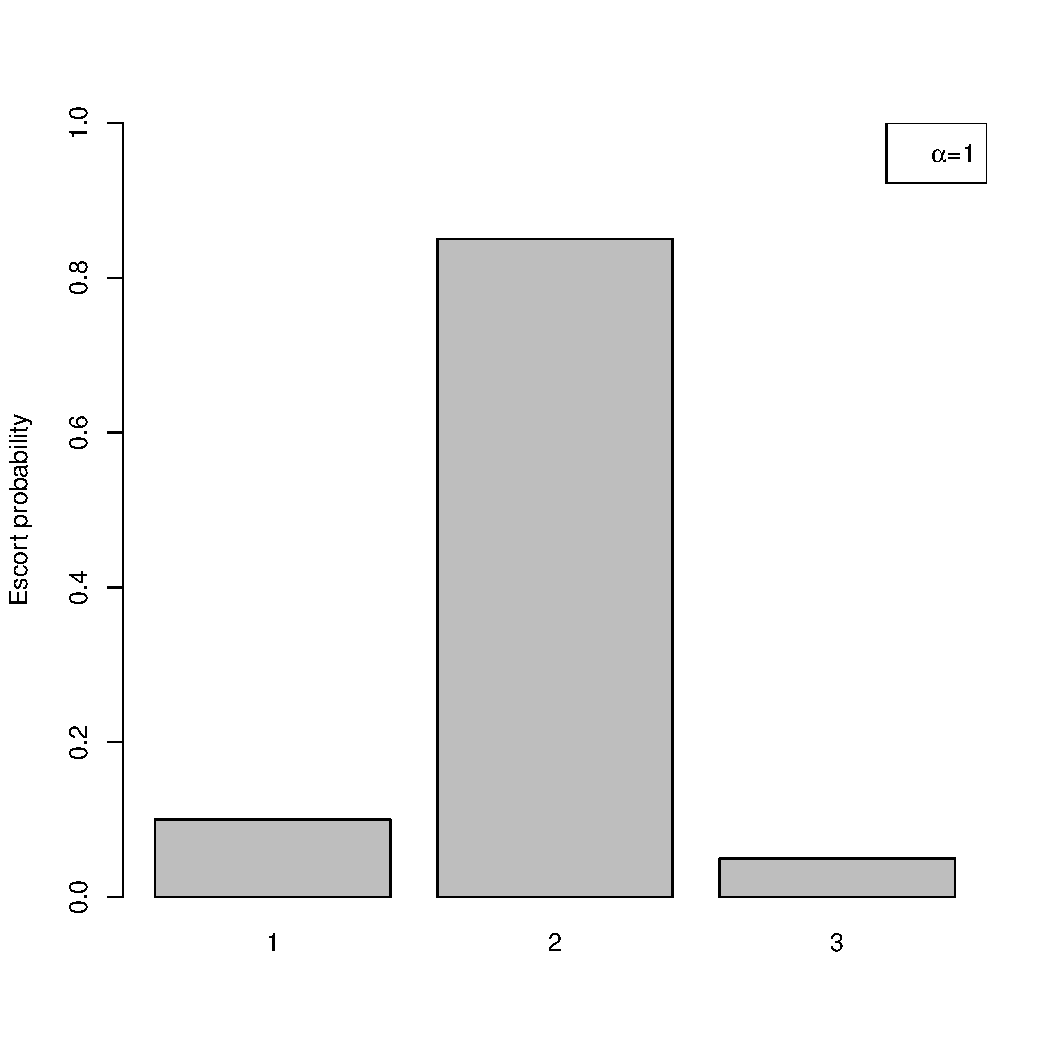
\includegraphics[trim=5mm 5mm 0 5mm,width=0.3\textwidth]{escort_fig1.pdf}
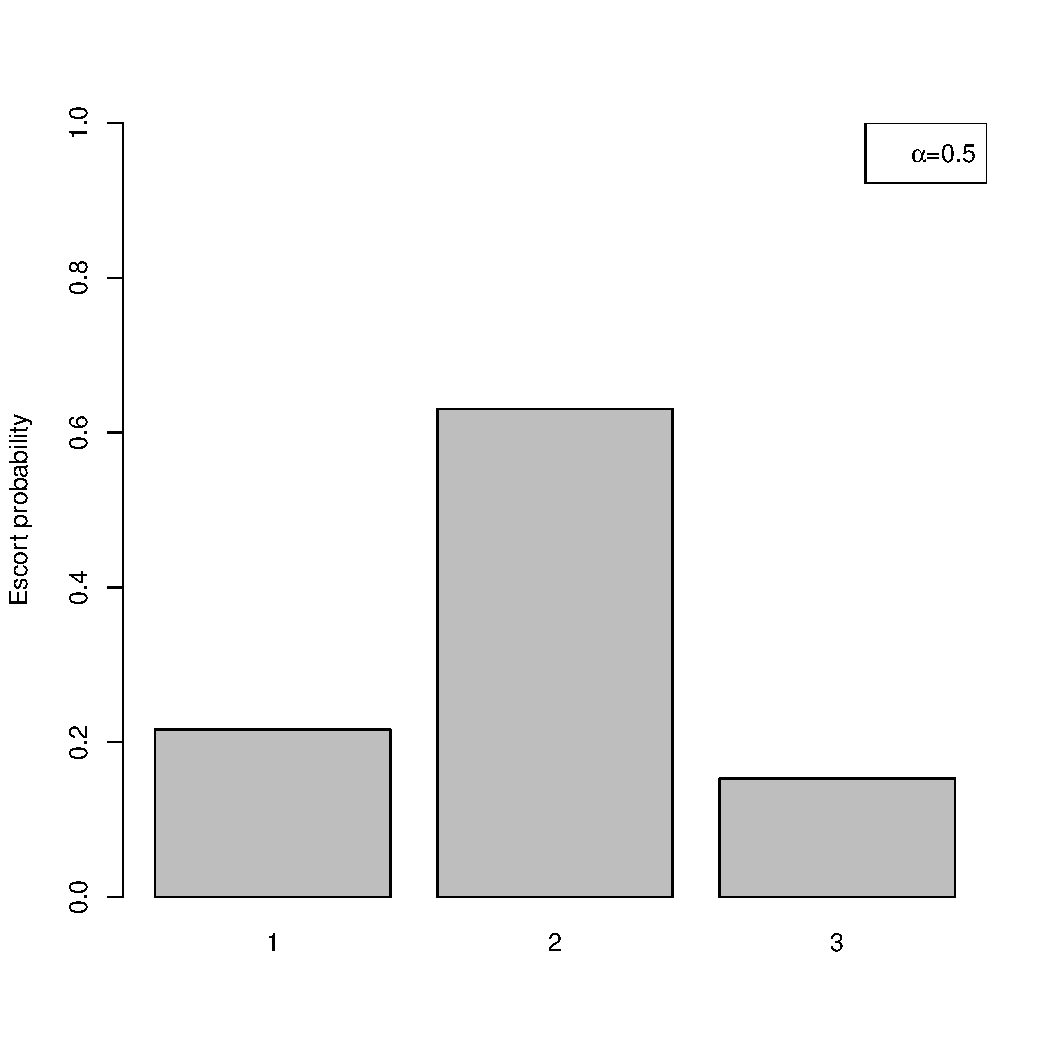
\includegraphics[trim=5mm 5mm 0 5mm,width=0.3\textwidth]{escort_fig2.pdf}
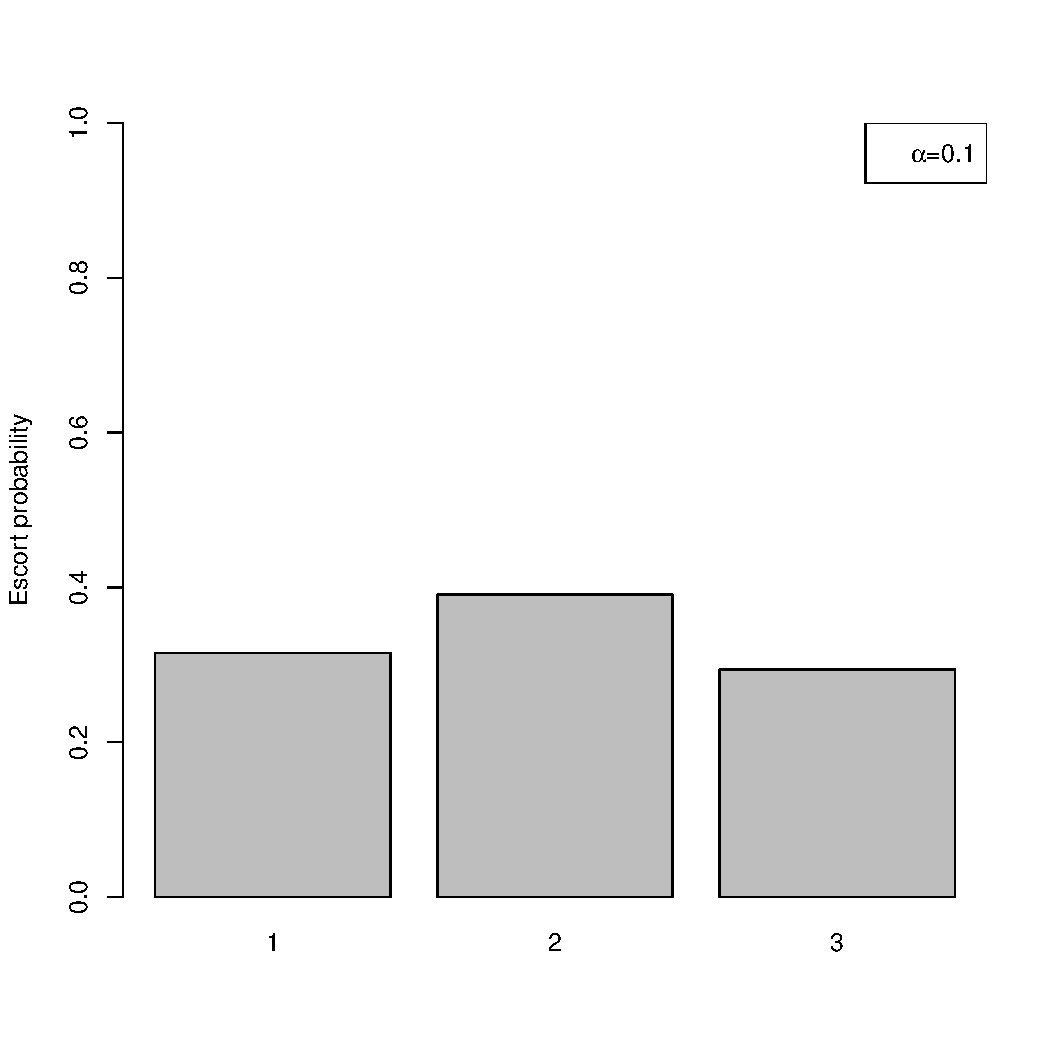
\includegraphics[trim=5mm 5mm 0 5mm,width=0.3\textwidth]{escort_fig3.pdf}
\caption{Escort distributions of $p(x)$.}
\end{figure}
\end{frame}
\begin{frame}{Best subset selection with unknown $k$}
\begin{itemize}\itemsep=3mm
\item We extend the proposed method to best subset selection with varying $k (<K)$, where $K$ is a pre-specified upper bound, $K<n$.
\item In our Bayesian framework, this extension can be easily done by assigning a prior for $k$.
\item Note that the uniform prior, $k \sim \text{Uniform}\{1,\ldots,K\}$, tends to assign larger probability to a larger subset. 
\item We define
$$\pi(k)\propto 1/\binom{p}{k} \mathbb{I}(k\leq K).$$
\end{itemize}
\end{frame}

\begin{frame}{Hybrid best subset search with varying $k$}
\begin{itemize}\itemsep=3mm
\item Bayesian best subset selection can be done by maximizing
$$ \pi(\bg,k|\uy) \propto f(\uy|\bg, k)\pi(\bg| k) \pi(k)$$
over $(\bg,k)$.
\item Our algorithm proceeds as follows:\\

 \begin{itemize}\itemsep=3mm
  \item[1.] \textbf{Repeat} for $k=1,\ldots,K$:
        \begin{itemize}
         \item[a.] Given $k$, implement the hybrid search algorithm.
         \item[b.] Set $\hat{\bg}_k=\hat{\bg}$.
        \end{itemize}
  \item[2.] Find $\hat{\bg}_{k_*}$ such that $$ \log f(\uy|\hat{\bg}_{k_*},{k_*})-\log \binom{p}{{k_*}} \geq \log f(\uy|\hat{\bg}_k,k)-\log \binom{p}{k},\quad \text{any $k\leq K$}.$$
 \end{itemize}

\end{itemize}
\end{frame}


\begin{frame}{Connection to extended BIC}

\begin{itemize}\itemsep=3mm
\item It can be shown that our posterior criterion is asymptotically equivalent to the extended BIC (EBIC) of \citet{chen2008extended}.
\item EBIC corresponds to the $L_0$-penalty sparse estimation with 
$$\lambda = \log (n)+ \frac{2}{k}\log \binom{p}{k}.$$
\end{itemize}
\end{frame}

\begin{frame}{Model selection consistency}

\begin{itemize}\itemsep=3mm
\item The proposed Bayesian approach possesses the model selection consistency in the high-dimensional setting with $p=p_n=O(n^\xi)$ for $\xi\geq 1$.
\item Hence, as $n\to \infty$, our variable selection procedure identifies the true model with probability tending to one.
\end{itemize}
\end{frame}


\begin{frame}{Simulation study}{Setup}
\begin{itemize}\itemsep=3mm
\item For given $n=100$, we generate the data from 
$$y_i\overset{ind}{\sim}\text{Normal}\left(\sum_{j=1}^p \beta_j x_{ij},1\right),$$
where 
\begin{itemize}\itemsep=3mm
\item $(x_{i1},\ldots,x_{ip})^\T \overset{iid}{\sim}\text{Normal}(\0_p,\uSigma)$ with $\uSigma=(\Sigma_{ij})_{p\times p}$ and $\Sigma_{ij}=\rho^{|i-j|}$,
\item $\beta_j \overset{iid}{\sim} \text{Uniform}\{-1,-2,1,2\}$ if $j\in \bg$ and $\beta_j=0$ if $j\notin \bg$. 
\item $\bg$ is an index set of size $4$ randomly selected from $\{1,2,\ldots,p\}$.
\item We consider four scenarios for $p$ and $\rho$: \\
(i) $p=200$, $\rho=0.1$, (ii) $p=200$, $\rho=0.9$,\\
 (iii) $p=1000$, $\rho=0.1$, (iv) $p=1000$, $\rho=0.9$. 
\end{itemize}
\end{itemize}
\end{frame}


\begin{frame}{Simulation study}{Results (high-dimensional scenarios)}
{\footnotesize
\begin{table}[H]
 \centering 
 \caption{MC size=$2,000$; FDR (false discovery rate), TRUE\% (percentage of the true model detected), SIZE (selected model size), HAM (Hamming distance).}\label{T:sim1}
 \begin{tabular}{cc|c|c|c|c}
  \hline
  Scenario & Method                         & FDR  (s.e.)    & TRUE\% (s.e.)   & SIZE (s.e.)     & HAM (s.e.)    \\
  \hline
i           & Proposed & 0.006 (0.001)  & 96.900 (0.388)  & 4.032 (0.004)    & 0.032 (0.004) \\
           & SCAD                           & 0.034 (0.002)  & 85.200 (0.794)  & 4.188 (0.011)   & 0.188 (0.011) \\
           & MCP                            & 0.035 (0.002)  & 84.750 (0.804)  & 4.191 (0.011)   & 0.191 (0.011) \\
           & ENET                           & 0.016 (0.001)  & 92.700 (0.582)  & 4.087 (0.007)   & 0.087 (0.007) \\
           & LASSO                          & 0.020 (0.002)  & 91.350 (0.629)  & 4.109 (0.009)   & 0.109 (0.009) \\
  \hline
ii           & Proposed & 0.023  (0.002) & 88.750  (0.707) & 3.985 (0.006)  & 0.203 (0.014) \\
           & SCAD                           & 0.059 (0.003)  & 74.150 (0.979)  & 4.107 (0.015)   & 0.480 (0.022) \\
           & MCP                            & 0.137 (0.004)  & 55.400 (1.112)  & 4.264 (0.020)   & 1.098 (0.034) \\
           & ENET                           & 0.501 (0.004)  & 0.300 (0.122)   & 7.716 (0.072)   & 5.018 (0.052) \\
           & LASSO                          & 0.276 (0.004)  & 15.550 (0.811)  & 5.308 (0.033)   & 2.038 (0.034) \\
  \hline
 \end{tabular}
\end{table}}
\end{frame}



\begin{frame}{Simulation study}{Results (ultra high-dimensional scenarios)}
{\footnotesize
\begin{table}[H]
 \centering 
 \caption{MC size=$2,000$; FDR (false discovery rate), TRUE\% (percentage of the true model detected), SIZE (selected model size), HAM (Hamming distance).}\label{T:sim2}
 \begin{tabular}{cc|c|c|c|c}
  \hline
  Scenario & Method                         & FDR  (s.e.)    & TRUE\% (s.e.)   & SIZE (s.e.)     & HAM (s.e.)    \\
  \hline
   iii        & Proposed & 0.004 (0.001)   & 98.100 (0.305)  & 4.020 (0.003)    & 0.020 (0.003) \\
           & SCAD                           & 0.027 (0.002)  & 87.900 (0.729)  & 4.145 (0.010)   & 0.145 (0.010) \\
           & MCP                            & 0.031 (0.002)  & 86.550 (0.763)  & 4.172 (0.013)   & 0.172 (0.013) \\
           & ENET                           & 0.035 (0.002)  & 84.850 (0.802)  & 4.181 (0.013)   & 0.206 (0.012) \\
           & LASSO                          & 0.014 (0.001)  & 93.850 (0.537)  & 4.073 (0.007)   & 0.073 (0.007) \\
  \hline
    iv       & Proposed & 0.023(0.002)   & 89.850 (0.675)  & 4.005 (0.005) & 0.190 (0.013) \\
           & SCAD                           & 0.068 (0.003)  & 74.250 (0.978)  & 4.196 (0.014)   & 0.493 (0.023) \\
           & MCP                            & 0.152 (0.004)  & 53.750 (1.115)  & 4.226 (0.017)   & 1.202 (0.035) \\
           & ENET                           & 0.417 (0.005)  & 0.150 (0.087)   & 6.228 (0.068)   & 4.089 (0.043) \\
           & LASSO                          & 0.265 (0.004)  & 19.500 (0.886)  & 5.139 (0.029)   & 1.909 (0.035) \\
  \hline
 \end{tabular}
\end{table}}
\end{frame}


\begin{frame}{Real data application}{Data description}
\begin{itemize}\itemsep=4mm
\item We apply the proposed method to Breast Invasive Carcinoma (BRCA) data generated by The Cancer Genome Atlas (TCGA) Research Network \url{http://cancergenome.nih.gov}. 
\item The data set is available at the \texttt{R} package \texttt{curatedTCGAData}. 
\item The data set contains $17,814$ gene expression measurements (recorded on the log scale) of $526$ patients with primary solid tumor. 
\item BRCA1 is a tumor suppressor gene and its mutations predispose women to breast cancer \citep{findlay2018accurate}. 
\item Our goal here is to identify the best fitting model for estimating an association between BRCA1 (response variable) and the other genes (independent variables). 

\end{itemize}
\end{frame}


\begin{frame}{Real data application}{Results (based on $4,000$ genes)}
\begin{table}[ht]
 \centering
 \caption{Model comparison}\label{T:realdata}
 \begin{tabular}{rrrrr}
  \hline
           & \# of selected  & PMSE & BIC     & EBIC    \\
  \hline
  Proposed & 8 & 0.60      & 984.45  & 1099.50 \\
  SCAD     & 4 & 0.68      & 1104.69 & 1166.47 \\
  MCP      & 4 & 0.68      & 1104.69 & 1166.47 \\
  ENET     & 5 & 0.68      & 1110.65 & 1186.25 \\
  LASSO    & 4 & 0.68      & 1104.69 & 1166.47 \\
  \hline
 \end{tabular}
\end{table}
\end{frame}
\begin{frame}{Real data application}{Results (cont.)}
\begin{figure}
 \centering
 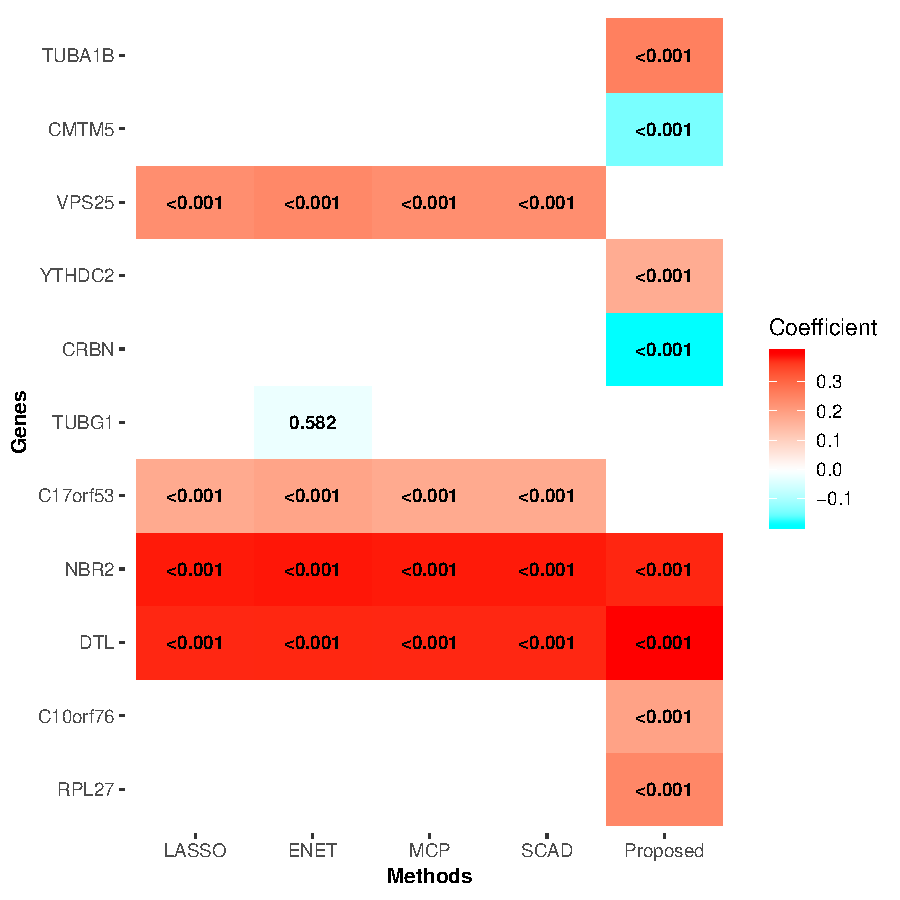
\includegraphics[width=0.6\textwidth,height=0.55\textwidth]{Heatmap.pdf}
 \caption{Except C10orf76, 7 genes are documented as \emph{diseases-related genes} }
\end{figure}

\end{frame}


\begin{frame}{Concluding remarks}
\begin{itemize}\itemsep=4mm
\item Parallel computing is applicable to our algorithm with varying $k$. 
\item The proposed method can be extended to multivariate linear regression models, binary regression models, and multivariate mixed responses models (in progress).
\end{itemize}

\end{frame}

\begin{frame}\footnotesize
%\bibliographystyle{biom}
%\bibliography{thesis_Goh}
\begin{thebibliography}{}
%\bibitem[\protect\citeauthoryear{Berg et al.}{Berg et al.}{2016}]{Berg:2016}
%Berg, E., Kim, J. K. and Skinner, C. (2016).
%\newblock Imputation under informative sampling
%\newblock {\em Journal of Survey Statistics and Methodology} {\bf }
%(In Press).

%\bibitem[\protect\citeauthoryear{Yin}{Yin}{2009}]{Yin:2009}
%Yin, G. (2009).
%\newblock Bayesian Generalized Method of Moments
%\newblock {\em Bayesian Analysis} {\bf 4,}
% 191--208.


%\bibitem[\protect\citeauthoryear{Xu, Chen and Mantel}{Xu, Chen and Mantel}{2013}]{Xu:2013}
%Xu, C., Chen, J., and Mantel, H. (2013).
%\newblock Pseudo-likelihood-based Bayesian information criterion for variable selection in survey data
%\newblock {\em Survey Methodology} {\bf 39,}
% 303--321.


%\bibitem[\protect\citeauthoryear{Li and Jiang}{Li and Jiang}{2014}]{Lin-Jiang:2014}
%Li, C. and Jiang, W. (2014).
%\newblock Model Selection for Likelihood-free Bayesian Methods Based on Moment Conditions: Theory and Numerical Examples
%\newblock {\em arXiv e-prints}.

%\bibitem[\protect\citeauthoryear{Schwarz}{Schwarz}{1978}]{Schwarz:1978}
%Schwarz, G. (1978).
%\newblock Estimating the dimension of a model.
%\newblock {\em The Annals of Statistics} {\bf 6,} 461--464.



\bibitem[\protect\citeauthoryear{Tibshirani}{Tibshirani}{1996}]{tibshirani1996regression}
Tibshirani, R. (1996).
\newblock Regression shrinkage and selection via the lasso.
\newblock {\em Journal of the Royal Statistical Society. Series B
  (Methodological)\/}, 267--288.


\bibitem[\protect\citeauthoryear{Hans, Dobra, and West}{Hans
  et~al.}{2007}]{hans2007shotgun}
Hans, C., A.~Dobra, and M.~West (2007).
\newblock Shotgun stochastic search for ``large p'' regression.
\newblock {\em Journal of the American Statistical Association\/}~{\em
  102\/}(478), 507--516.


\bibitem[\protect\citeauthoryear{Chen and Chen}{Chen and
  Chen}{2008}]{chen2008extended}
Chen, J. and Z.~Chen (2008).
\newblock Extended bayesian information criteria for model selection with large
  model spaces.
\newblock {\em Biometrika\/}~{\em 95\/}(3), 759--771.


\bibitem[\protect\citeauthoryear{Findlay, Daza, Martin, Zhang, Leith,
  Gasperini, Janizek, Huang, Starita, and Shendure}{Findlay
  et~al.}{2018}]{findlay2018accurate}
Findlay, G.~M., R.~M. Daza, B.~Martin, M.~D. Zhang, A.~P. Leith, M.~Gasperini,
  J.~D. Janizek, X.~Huang, L.~M. Starita, and J.~Shendure (2018).
\newblock Accurate classification of brca1 variants with saturation genome
  editing.
\newblock {\em Nature\/}~{\em 562\/}(7726), 217.

\end{thebibliography}
\end{frame}
%\bibliography{thesis_Goh}

\begin{frame}{Q/A}\vspace{2mm}
\centering \huge THANK YOU
\end{frame}

\end{document}



